
\documentclass[12pt,a4paper]{article}

% ------------------------------------------------------------
% Fonts & layout
% ------------------------------------------------------------
\usepackage[T1]{fontenc}
\usepackage[utf8]{inputenc}
\usepackage{lmodern}
\usepackage{microtype}
\usepackage{geometry}
\geometry{margin=1in}
\usepackage{array}
\usepackage{booktabs}

% ------------------------------------------------------------
% Math
% ------------------------------------------------------------
\usepackage{amsmath,amssymb,amsthm,mathtools}

% Standard operators
\DeclareMathOperator{\id}{id}
\DeclareMathOperator{\im}{im}
\DeclareMathOperator{\coker}{coker}
\DeclareMathOperator{\Hom}{Hom}

\DeclareMathOperator{\Spec}{Spec}
\DeclareMathOperator{\Proj}{Proj}

% Categories / notation
\newcommand{\Ab}{\mathbf{Ab}}
\newcommand{\PreSh}{\mathbf{PreSh}}
\newcommand{\Sh}{\mathbf{Sh}}

\newcommand{\F}{\mathcal F}


% basic number sets
\newcommand{\RR}{\mathbb{R}}

% sheaf letters

\newcommand{\G}{\mathcal G}

\newcommand{\GG}{\mathbb G}


\newcommand{\AffSch}{\mathbf{AffSch}}
\newcommand{\ZZ}{\mathbb Z}

\newcommand{\PP}{\mathbb P}

\usepackage{tikz}
\usetikzlibrary{decorations.pathreplacing}
\usetikzlibrary{positioning,arrows.meta}

% sheaf of continuous real-valued functions
\newcommand{\Czero}{\mathcal C^0}        % “C^0”
\newcommand{\CzeroX}{\mathcal C^0_X}     % sheaf on X (optional)

\newcommand{\Cinfty}{\mathcal C^\infty}
\newcommand{\CinftyM}{\mathcal C^\infty_M} % if you use C^\infty_M

% number sets / standard symbols
\newcommand{\CC}{\mathbb{C}}

% structure sheaf notation in complex geometry
\newcommand{\OO}{\mathcal{O}}
\newcommand{\OOX}{\mathcal{O}_X} % optional convenience



\newcommand{\Sch}{\mathrm{Sch}}
\newcommand{\Rings}{\mathrm{Rings}}

\newcommand{\kappares}{\kappa}
\newcommand{\GammaX}{\Gamma(X,\mathcal O_X)}

\newtheorem{theorem}{Theorem}[section]
\newtheorem{proposition}[theorem]{Proposition}
\newtheorem{lemma}[theorem]{Lemma}

\newcommand{\nilrad}{\sqrt{(0)}}

\newcommand{\Frac}{\operatorname{Frac}}
\newcommand{\codim}{\operatorname{codim}}
\newcommand{\trdeg}{\operatorname{trdeg}}

\newcommand{\height}{\operatorname{height}}

\newcommand{\Pic}{\operatorname{Pic}}
\newcommand{\divisor}{\operatorname{div}}

\newcommand{\Z}{\mathbb{Z}}
\newcommand{\Cl}{\operatorname{Cl}}

\providecommand{\Spec}{\operatorname{Spec}}
\providecommand{\A}{\mathbb A}
\providecommand{\Pj}{\mathbb P}
\providecommand{\G}{\mathbb G}

% ------------------------------------------------------------
% Links
% ------------------------------------------------------------
\usepackage{xcolor}
\usepackage{hyperref}
\usepackage{bookmark}
\hypersetup{
  colorlinks=true,
  linkcolor=blue!50!black,
  urlcolor=blue!50!black,
  citecolor=blue!50!black,
  pdftitle={Algebraic Geometry 9
  },
  pdfauthor={},
  pdfsubject={Lecture notes (reorganized)},
  pdfcreator={TeXStudio / LaTeX}
}

% ------------------------------------------------------------
% Diagrams
% ------------------------------------------------------------
\usepackage{tikz-cd}

% ------------------------------------------------------------
% Lists
% ------------------------------------------------------------
\usepackage{enumitem}
\setlist[itemize]{topsep=4pt,itemsep=2pt,parsep=0pt,partopsep=0pt}
\setlist[enumerate]{topsep=4pt,itemsep=2pt,parsep=0pt,partopsep=0pt}

% ------------------------------------------------------------
% Theorem environments
% ------------------------------------------------------------
\newtheoremstyle{notespace}{6pt}{6pt}{\normalfont}{}{\bfseries}{.}{0.5em}{}
\theoremstyle{notespace}
\newtheorem{definition}{Definition}[subsection]

\newtheorem{corollary}[definition]{Corollary}
\newtheorem{remark}[definition]{Remark}
\newtheorem{example}[definition]{Example}
\newtheorem{warning}[definition]{Warning}




\newcommand{\B}{\mathcal B}
\newcommand{\C}{\mathcal C}
\newcommand{\Ocal}{\mathcal O}
\newcommand{\I}{\mathcal I}


\newcommand{\Fp}{\mathcal F'}      % subsheaf
\newcommand{\Fpp}{\mathcal F''} 

\newcommand{\GammaU}[1]{\Gamma(U,#1)}

\DeclareMathOperator*{\colim}{colim}

% circle
\newcommand{\SSone}{S^1}


\usetikzlibrary{arrows.meta,positioning,calc,shapes.geometric,fit}

\usepackage{adjustbox}

% sheaves of continuous functions


% ------------------------------------------------------------
% Paragraph spacing
% ------------------------------------------------------------
\setlength{\parskip}{0.5em}
\setlength{\parindent}{0pt}

\setcounter{tocdepth}{2}
\setcounter{secnumdepth}{2}

% ------------------------------------------------------------
% Fancy headers
% ------------------------------------------------------------
\usepackage{fancyhdr}
\pagestyle{fancy}
\fancyhf{}
\lhead{Theory of Algebraic Geometry 12}
\rhead{\thepage}
\renewcommand{\headrulewidth}{0.4pt}
\setlength{\headheight}{14.5pt}




\begin{document}


\title{Algebraic Geometry 12\\
	\large Riemann surfaces}
\author{}
\date{}

	\maketitle
	

	\setcounter{section}{0}

\tableofcontents

	\clearpage
	
	
\section*{Problem}

Let \(\Lambda\subset \mathbb C\) be a lattice and let \(\wp=\wp_\Lambda\) be the Weierstrass function.

\subsection*{(i) Every analytic function on \(\mathbb C/\Lambda\setminus\{0\}\)}

Let \(f\) be analytic on \(\mathbb C/\Lambda\setminus\{0\}\).  
Equivalently, \(f\) is an elliptic function on \(\mathbb C\) whose only possible pole is at lattice points.

Since \(f\) is elliptic, it has a Laurent expansion at \(0\):

\[
f(z)=\sum_{n=-N}^{\infty} a_n z^n.
\]

We use the basic expansions

\[
\wp(z)=\frac{1}{z^2}+O(z^2),
\qquad
\wp'(z)=-\frac{2}{z^3}+O(z).
\]

Thus powers of \(\wp\) produce even principal parts:

\[
\wp(z)^k=\frac{1}{z^{2k}}+\cdots,
\]

and \(\wp'(z)\wp(z)^k\) produces odd principal parts:

\[
\wp'(z)\wp(z)^k=-\frac{2}{z^{2k+3}}+\cdots.
\]

Therefore we can subtract a polynomial in \(\wp\) and \(\wp'\) from \(f\) so that all negative terms in the Laurent expansion disappear.

So there exists

\[
P(X,Y)\in \mathbb C[X,Y]
\]

such that

\[
g(z)=f(z)-P(\wp(z),\wp'(z))
\]

has no pole at \(0\). Hence \(g\) is holomorphic on all of \(\mathbb C/\Lambda\).

But \(\mathbb C/\Lambda\) is compact, so every holomorphic function on it is constant. Hence

\[
g(z)=c.
\]

Therefore

\[
f(z)=P(\wp(z),\wp'(z))+c.
\]

Absorbing \(c\) into the polynomial, we get

\[
f(z)\in \mathbb C[\wp(z),\wp'(z)].
\]

Thus every analytic function on \(\mathbb C/\Lambda\setminus\{0\}\) is a polynomial in \(\wp(z)\) and \(\wp'(z)\).

\[
\boxed{
	\mathcal O(\mathbb C/\Lambda\setminus\{0\})
	=
	\mathbb C[\wp,\wp']
}
\]

\subsection*{(ii) The only polynomial relation}

The Weierstrass function satisfies

\[
(\wp'(z))^2
=
4(\wp(z)-e_1)(\wp(z)-e_2)(\wp(z)-e_3),
\]

where

\[
e_i=\wp(\omega_i/2).
\]

Thus

\[
Y^2-4\prod_{i=1}^3(X-e_i)
\]

certainly vanishes after substituting

\[
X=\wp(z),
\qquad
Y=\wp'(z).
\]

Now suppose

\[
F(X,Y)\in \mathbb C[X,Y]
\]

satisfies

\[
F(\wp(z),\wp'(z))=0
\]

for all \(z\).

Let

\[
R(X,Y)=Y^2-4\prod_{i=1}^3(X-e_i).
\]

Since \(R\) is monic in \(Y\), divide \(F\) by \(R\) as a polynomial in \(Y\):

\[
F(X,Y)=Q(X,Y)R(X,Y)+A(X)Y+B(X),
\]

where

\[
A(X),B(X)\in \mathbb C[X].
\]

Substituting \(X=\wp(z)\), \(Y=\wp'(z)\), and using \(R(\wp,\wp')=0\), we get

\[
A(\wp(z))\wp'(z)+B(\wp(z))=0.
\]

Now replace \(z\) by \(-z\). Since

\[
\wp(-z)=\wp(z),
\qquad
\wp'(-z)=-\wp'(z),
\]

we also get

\[
-A(\wp(z))\wp'(z)+B(\wp(z))=0.
\]

Adding and subtracting the two equations gives

\[
B(\wp(z))=0,
\qquad
A(\wp(z))\wp'(z)=0.
\]

Since \(\wp\) is nonconstant, \(B(\wp(z))=0\) implies

\[
B=0.
\]

Also \(\wp'\not\equiv 0\), so

\[
A(\wp(z))=0,
\]

and again since \(\wp\) is nonconstant,

\[
A=0.
\]

Therefore the remainder is zero, so

\[
F(X,Y)=Q(X,Y)R(X,Y).
\]

Hence

\[
F(X,Y)
\]

is a multiple of

\[
Y^2-4\prod_{i=1}^3(X-e_i).
\]

Therefore

\[
\boxed{
	F\in
	\left(
	Y^2-4\prod_{i=1}^3(X-e_i)
	\right).
}
\]

So the kernel of the map

\[
\mathbb C[X,Y]\longrightarrow \mathcal O(\mathbb C/\Lambda\setminus\{0\}),
\qquad
X\mapsto \wp,
\quad
Y\mapsto \wp'
\]

is exactly

\[
\boxed{
	\left(
	Y^2-4\prod_{i=1}^3(X-e_i)
	\right).
}
\]
	
\section{The Lattice \(\Lambda\), Periods \(\omega_1,\omega_2\), and the Weierstrass Function}

To construct the Weierstrass elliptic function, we begin with two complex numbers

\[
\omega_1,\omega_2\in\mathbb C
\]

which are linearly independent over \(\mathbb R\). Equivalently,

\[
\frac{\omega_1}{\omega_2}\notin\mathbb R.
\]

For example,

\[
\omega_1=1,
\qquad
\omega_2=i.
\]

\subsection{The Lattice}

The lattice generated by \(\omega_1\) and \(\omega_2\) is

\[
\Lambda
=
\mathbb Z\omega_1+\mathbb Z\omega_2
=
\{
m\omega_1+n\omega_2
:
m,n\in\mathbb Z
\}.
\]

In the example \(\omega_1=1\) and \(\omega_2=i\),

\[
\Lambda
=
\{
m+ni
:
m,n\in\mathbb Z
\},
\]

which is the integer grid in the complex plane.

The points of \(\Lambda\) form a discrete subgroup of \(\mathbb C\).

\subsection{Fundamental Parallelogram}

The lattice determines a fundamental parallelogram

\[
P=
\{
a\omega_1+b\omega_2
:
0\le a,b<1
\}.
\]

Every point of \(\mathbb C\) can be translated by a lattice vector into \(P\).

\begin{center}
	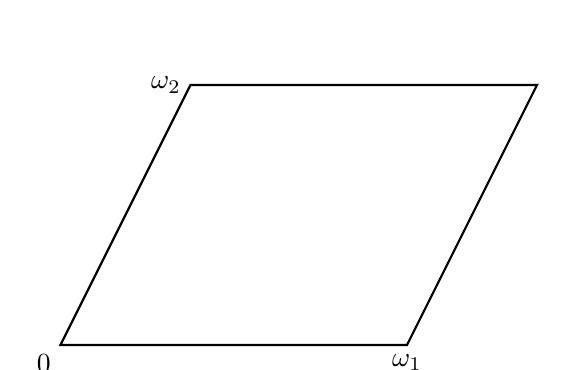
\begin{tikzpicture}[scale=1.1]
		
		\coordinate (O) at (0,0);
		\coordinate (A) at (4,0);
		\coordinate (B) at (1.5,3);
		\coordinate (C) at (5.5,3);
		
		\draw[thick] (O)--(A)--(C)--(B)--cycle;
		
		\node[below] at (A) {$\omega_1$};
		\node[left] at (B) {$\omega_2$};
		\node[below left] at (O) {$0$};
		
	\end{tikzpicture}
\end{center}

\subsection{The Quotient \(\mathbb C/\Lambda\)}

Two points are considered equivalent if they differ by a lattice vector:

\[
z\sim z+\lambda,
\qquad
\lambda\in\Lambda.
\]

Thus

\[
0,
\quad
\omega_1,
\quad
\omega_2,
\quad
\omega_1+\omega_2
\]

all represent the same point in the quotient.

The quotient space

\[
\mathbb C/\Lambda
\]

is obtained by identifying opposite sides of the fundamental parallelogram.

Topologically,

\[
\boxed{\mathbb C/\Lambda \cong \text{torus}.}
\]

\subsection{The Weierstrass Function}

The Weierstrass function associated with \(\Lambda\) is

\[
\wp(z)
=
\frac{1}{z^2}
+
\sum_{\omega\in\Lambda\setminus\{0\}}
\left(
\frac{1}{(z-\omega)^2}
-
\frac{1}{\omega^2}
\right).
\]

It satisfies

\[
\wp(z+\lambda)=\wp(z)
\qquad
(\lambda\in\Lambda).
\]

Therefore \(\wp\) descends to a meromorphic function on the torus

\[
\mathbb C/\Lambda.
\]

Its derivative

\[
\wp'(z)
=
-2
\sum_{\omega\in\Lambda}
\frac{1}{(z-\omega)^3}
\]

is also elliptic.

\subsection{Half-Periods}

The three nonzero half-periods are

\[
\frac{\omega_1}{2},
\qquad
\frac{\omega_2}{2},
\qquad
\frac{\omega_1+\omega_2}{2}.
\]

These are special points on the torus.

A fundamental theorem states that

\[
\wp'(z)=0
\]

precisely at these three half-periods (modulo \(\Lambda\)).

\subsection{The Numbers \(e_1,e_2,e_3\)}

Define

\[
e_1
=
\wp\!\left(\frac{\omega_1}{2}\right),
\]

\[
e_2
=
\wp\!\left(\frac{\omega_2}{2}\right),
\]

\[
e_3
=
\wp\!\left(\frac{\omega_1+\omega_2}{2}\right).
\]

These numbers are the roots of the cubic polynomial appearing in the fundamental differential equation of \(\wp\).

\subsection{The Fundamental Relation}

The Weierstrass function satisfies

\[
(\wp'(z))^2
=
4(\wp(z)-e_1)
(\wp(z)-e_2)
(\wp(z)-e_3).
\]

This relation shows that the pair

\[
(\wp(z),\wp'(z))
\]

lies on the affine elliptic curve

\[
\boxed{
	Y^2
	=
	4(X-e_1)(X-e_2)(X-e_3).
}
\]

Consequently,

\[
\mathbb C/\Lambda
\]

can be viewed geometrically as this elliptic curve, with coordinates

\[
X=\wp(z),
\qquad
Y=\wp'(z).
\]

\subsection{Concrete Example}

Let

\[
\Lambda
=
\mathbb Z+\mathbb Zi.
\]

Then

\[
\omega_1=1,
\qquad
\omega_2=i.
\]

The half-periods are

\[
\frac12,
\qquad
\frac{i}{2},
\qquad
\frac{1+i}{2}.
\]

The corresponding values are

\[
e_1=\wp\!\left(\frac12\right),
\qquad
e_2=\wp\!\left(\frac{i}{2}\right),
\qquad
e_3=\wp\!\left(\frac{1+i}{2}\right).
\]

The associated elliptic curve is

\[
Y^2
=
4(X-e_1)(X-e_2)(X-e_3).
\]

Thus the construction proceeds through the chain

\[
\omega_1,\omega_2
\Longrightarrow
\Lambda
\Longrightarrow
\wp_\Lambda
\Longrightarrow
e_1,e_2,e_3
\Longrightarrow
Y^2=4(X-e_1)(X-e_2)(X-e_3).
\]

\section{Problem 2}

Let \(a\in\mathbb C\) satisfy \(|a|>1\). Suppose

\[
f(az)=f(z)
\]

for all \(z\in\mathbb C^*=\mathbb C\setminus\{0\}\).

Show that every analytic such function is constant, but that there exists a non-constant meromorphic such function.

\subsection{Part (i): Analytic Functions}

Assume \(f\) is analytic on \(\mathbb C^*\) and satisfies

\[
f(az)=f(z).
\]

Since \(f\) is analytic on \(\mathbb C^*\), it admits a Laurent expansion

\[
f(z)=\sum_{n=-\infty}^{\infty} c_n z^n.
\]

Substituting \(az\) gives

\[
f(az)
=
\sum_{n=-\infty}^{\infty}
c_n a^n z^n.
\]

Since \(f(az)=f(z)\), comparison of coefficients yields

\[
c_n(a^n-1)=0
\]

for every integer \(n\).

Because \(|a|>1\), we have

\[
a^n\neq 1
\]

for all \(n\neq 0\).

Hence

\[
c_n=0
\qquad (n\neq 0).
\]

Therefore only the constant coefficient survives:

\[
f(z)=c_0.
\]

Thus every analytic solution is constant.

\[
\boxed{
	f(z)\equiv \text{constant}.
}
\]

\subsection{Part (ii): A Non-Constant Meromorphic Solution}

Let

\[
u=
\frac{2\pi i}{\log a}\log z.
\]

Then

\[
z\mapsto az
\]

induces

\[
u\mapsto u+2\pi i.
\]

The cotangent function is periodic:

\[
\cot(u+2\pi i)=\cot(u).
\]

Hence

\[
f(z)
=
\cot\!\left(
\frac{2\pi i}{\log a}\log z
\right)
\]

satisfies

\[
f(az)=f(z).
\]

Since \(\cot\) is non-constant and meromorphic, this gives a non-constant meromorphic solution.

\[
\boxed{
	f(z)
	=
	\cot\!\left(
	\frac{2\pi i}{\log a}\log z
	\right).
}
\]

\subsection{Conclusion}

Every analytic solution is constant, whereas non-constant meromorphic solutions exist.

\[
\boxed{
	\text{Analytic } \Rightarrow \text{constant},
	\qquad
	\text{Meromorphic } \not\Rightarrow \text{constant}.
}
\]

\newpage

\section{Problem 3}

Let \(\wp(z)\) be the Weierstrass elliptic function associated with a lattice \(\Lambda\).

Show that

\[
\wp''(z)=6\wp(z)^2+A
\]

for some constant \(A\in\mathbb C\).

Then show that there are at least three and at most five points modulo \(\Lambda\) at which \(\wp'\) is not locally injective.

\subsection{Part (i): Computing \(\wp''\)}

The Weierstrass function satisfies

\[
(\wp'(z))^2
=
4\wp(z)^3-g_2\wp(z)-g_3.
\]

Differentiating both sides yields

\[
2\wp'(z)\wp''(z)
=
\bigl(12\wp(z)^2-g_2\bigr)\wp'(z).
\]

At points where \(\wp'(z)\neq 0\), dividing by \(2\wp'(z)\) gives

\[
\wp''(z)
=
6\wp(z)^2-\frac{g_2}{2}.
\]

Since both sides are meromorphic and agree on a dense set, they agree everywhere.

Thus

\[
\boxed{
	\wp''(z)
	=
	6\wp(z)^2+A
}
\]

where

\[
A=-\frac{g_2}{2}.
\]

\subsection{Part (ii): Failure of Local Injectivity}

A holomorphic map fails to be locally injective precisely at points where its derivative vanishes.

For the function

\[
\wp'(z),
\]

the derivative is

\[
(\wp')'(z)=\wp''(z).
\]

Hence \(\wp'\) is not locally injective exactly when

\[
\wp''(z)=0.
\]

Using the formula above,

\[
6\wp(z)^2+A=0.
\]

Therefore

\[
\wp(z)^2
=
-\frac{A}{6}.
\]

Let

\[
c^2
=
-\frac{A}{6}.
\]

Then every critical point satisfies

\[
\wp(z)=c
\]

or

\[
\wp(z)=-c.
\]

\subsection{Counting the Solutions}

The map

\[
\wp:\mathbb C/\Lambda\to\mathbb P^1
\]

has degree \(2\).

Therefore each value of \(\wp\) has at most two preimages modulo \(\Lambda\).

Since the equation

\[
\wp(z)^2=c^2
\]

corresponds to the two values \(c\) and \(-c\), there are at most four solutions in the generic case.

Allowing multiplicities and possible branch points gives at most five distinct points modulo \(\Lambda\).

Thus

\[
\boxed{
	\text{at most five points modulo }\Lambda.
}
\]

To obtain a lower bound, observe that \(\wp'\) is a non-constant elliptic function. By the Riemann--Hurwitz theorem applied to

\[
\wp':\mathbb C/\Lambda\to\mathbb P^1,
\]

the total ramification is positive. Consequently \(\wp'\) must possess several critical points.

In particular there cannot be fewer than three distinct critical points modulo \(\Lambda\).

Hence

\[
\boxed{
	\text{at least three points modulo }\Lambda.
}
\]

\subsection{Conclusion}

The second derivative of the Weierstrass function is

\[
\boxed{
	\wp''(z)
	=
	6\wp(z)^2-\frac{g_2}{2}.
}
\]

The critical points of \(\wp'\) are the solutions of

\[
6\wp(z)^2-\frac{g_2}{2}=0,
\]

and therefore \(\wp'\) fails to be locally injective at

\[
\boxed{
	\text{at least three and at most five points modulo }\Lambda.
}
\]
	
	
\section{Theoretical Background: Elliptic Functions, Quotients, and Ramification}

These exercises illustrate three fundamental themes in complex analysis and the theory of elliptic curves:

\begin{enumerate}
	\item Elliptic functions as algebraic functions on an elliptic curve.
	\item Analytic and meromorphic functions on quotient Riemann surfaces.
	\item Critical points and ramification of holomorphic maps.
\end{enumerate}

\subsection{1. Elliptic Functions and Lattices}

Let

\[
\Lambda=\mathbb Z\omega_1+\mathbb Z\omega_2
\]

be a lattice in \(\mathbb C\), where

\[
\frac{\omega_1}{\omega_2}\notin\mathbb R.
\]

The quotient

\[
E=\mathbb C/\Lambda
\]

is a compact Riemann surface of genus one.

Topologically, \(E\) is a torus.

Functions on \(E\) correspond to doubly-periodic functions on \(\mathbb C\):

\[
f(z+\lambda)=f(z)
\qquad
(\lambda\in\Lambda).
\]

Such functions are called elliptic functions.

\subsection{2. The Weierstrass Function}

The basic elliptic function associated with \(\Lambda\) is

\[
\wp(z)
=
\frac{1}{z^2}
+
\sum_{\omega\in\Lambda\setminus\{0\}}
\left(
\frac{1}{(z-\omega)^2}
-
\frac{1}{\omega^2}
\right).
\]

Its derivative is

\[
\wp'(z).
\]

The functions satisfy

\[
(\wp')^2
=
4\wp^3-g_2\wp-g_3.
\]

Consequently the pair

\[
(\wp(z),\wp'(z))
\]

lies on the cubic curve

\[
Y^2
=
4X^3-g_2X-g_3.
\]

Equivalently,

\[
Y^2
=
4(X-e_1)(X-e_2)(X-e_3).
\]

Thus the torus \(E\) acquires an algebraic description as an elliptic curve.

\subsection{3. The Coordinate Ring of the Punctured Torus}

Removing the origin gives

\[
E\setminus\{0\}.
\]

The point \(0\) is the unique pole of \(\wp\).

Every holomorphic function on

\[
E\setminus\{0\}
\]

can only have a pole at \(0\).

Because \(\wp\) and \(\wp'\) generate all possible principal parts at \(0\), one obtains

\[
\mathcal O(E\setminus\{0\})
=
\mathbb C[\wp,\wp'].
\]

This is analogous to the fact that

\[
\mathbb C[x]
\]

is the ring of regular functions on the affine line.

The relation

\[
(\wp')^2
=
4(\wp-e_1)(\wp-e_2)(\wp-e_3)
\]

shows that

\[
\mathbb C[\wp,\wp']
\cong
\frac{
	\mathbb C[X,Y]
}{
	(Y^2-4(X-e_1)(X-e_2)(X-e_3))
}.
\]

Thus the punctured torus is identified with an affine elliptic curve.

\subsection{4. Multiplicative Quotients and Periodicity}

Exercise 2 concerns the multiplicative action

\[
z\mapsto az
\]

with

\[
|a|>1.
\]

Repeated multiplication generates the infinite cyclic group

\[
a^{\mathbb Z}.
\]

The quotient

\[
\mathbb C^*/a^{\mathbb Z}
\]

is again a complex torus.

Indeed, writing

\[
z=e^w
\]

transforms multiplication into translation:

\[
w\mapsto w+\log a.
\]

Hence

\[
\mathbb C^*
=
\mathbb C/(2\pi i\mathbb Z)
\]

and further quotienting by

\[
\log a
\]

produces a lattice

\[
2\pi i\mathbb Z+\log(a)\mathbb Z.
\]

Therefore

\[
\mathbb C^*/a^{\mathbb Z}
\]

is an elliptic curve.

The statement that every analytic function satisfying

\[
f(az)=f(z)
\]

is constant reflects the compactness of the quotient.

However, meromorphic functions exist because compact Riemann surfaces always admit nonconstant meromorphic functions.

\subsection{5. Critical Points and Local Injectivity}

Let

\[
f:X\to Y
\]

be a holomorphic map between Riemann surfaces.

A point \(p\in X\) is critical if

\[
f'(p)=0.
\]

At such points the map fails to be locally injective.

For

\[
f=\wp',
\]

the critical points are solutions of

\[
\wp''(z)=0.
\]

Differentiating the fundamental equation gives

\[
\wp''(z)
=
6\wp(z)^2-\frac{g_2}{2}.
\]

Thus critical points satisfy

\[
\wp(z)^2
=
\frac{g_2}{12}.
\]

Because

\[
\wp:E\to\mathbb P^1
\]

has degree \(2\), every value has at most two preimages.

This immediately yields strong bounds on the number of critical points.

\subsection{6. Ramification Theory}

Critical points are measured globally by the Riemann--Hurwitz formula.

If

\[
f:X\to Y
\]

has degree \(d\), then

\[
2g_X-2
=
d(2g_Y-2)
+
\sum_{p\in X}(e_p-1),
\]

where \(e_p\) is the ramification index.

For

\[
\wp':E\to\mathbb P^1,
\]

we have

\[
g(E)=1,
\qquad
g(\mathbb P^1)=0.
\]

Hence

\[
0
=
-2d
+
\sum (e_p-1).
\]

This forces the existence of critical points.

The lower and upper bounds obtained in Exercise 3 are manifestations of this global ramification constraint.

\subsection{7. Geometric Interpretation}

The three exercises together establish the following picture:

\[
\Lambda
\longrightarrow
E=\mathbb C/\Lambda
\longrightarrow
(\wp,\wp')
\longrightarrow
Y^2=4(X-e_1)(X-e_2)(X-e_3).
\]

The torus becomes an algebraic curve.

Functions on the torus become rational functions in \(\wp\) and \(\wp'\).

Critical points correspond to ramification points of the map to the projective line.

Thus complex analysis, algebraic geometry, and topology meet naturally in the theory of elliptic curves.

\section{Examples and Detailed Calculations}

\subsection{Example 1: A Concrete Lattice and Torus}

Consider the lattice

\[
\Lambda=\mathbb Z+\mathbb Zi.
\]

Thus the fundamental periods are

\[
\omega_1=1,
\qquad
\omega_2=i.
\]

The lattice points are

\[
0,\pm1,\pm i,\pm(1+i),\pm(2+i),\ldots
\]

\subsubsection*{Step 1: Construct a Fundamental Domain}

A fundamental parallelogram is

\[
P=
\{
x+iy
:
0\le x<1,\;
0\le y<1
\}.
\]

In this case it is simply the unit square.

\begin{center}
	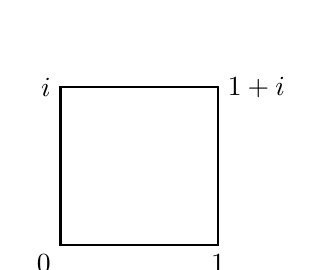
\begin{tikzpicture}[scale=2]
		
		\draw[thick] (0,0) rectangle (1,1);
		
		\node[below left] at (0,0) {$0$};
		\node[below] at (1,0) {$1$};
		\node[left] at (0,1) {$i$};
		\node[right] at (1,1) {$1+i$};
		
	\end{tikzpicture}
\end{center}

\subsubsection*{Step 2: Identify Opposite Sides}

We identify

\[
(x,0)\sim(x,1)
\]

and

\[
(0,y)\sim(1,y).
\]

First gluing one pair of opposite sides produces a cylinder.

Gluing the remaining pair produces a torus.

Therefore

\[
\boxed{
	\mathbb C/\Lambda
	\cong
	\text{torus}.
}
\]

\subsubsection*{Step 3: Equivalent Points}

The points

\[
z,
\quad
z+1,
\quad
z+i,
\quad
z+1+i
\]

all represent the same point on the torus.

For example,

\[
0.3+0.2i
\]

and

\[
1.3+2.2i
\]

differ by

\[
1+2i\in\Lambda,
\]

hence represent the same point of

\[
\mathbb C/\Lambda.
\]

\bigskip

\subsection{Example 2: From the Torus to an Elliptic Curve}

Using the same lattice

\[
\Lambda=\mathbb Z+\mathbb Zi,
\]

consider the Weierstrass function \(\wp(z)\).

Define

\[
e_1=
\wp\!\left(\frac12\right),
\qquad
e_2=
\wp\!\left(\frac{i}{2}\right),
\qquad
e_3=
\wp\!\left(\frac{1+i}{2}\right).
\]

\subsubsection*{Step 1: Fundamental Relation}

The Weierstrass function satisfies

\[
(\wp'(z))^2
=
4(\wp(z)-e_1)
(\wp(z)-e_2)
(\wp(z)-e_3).
\]

\subsubsection*{Step 2: Introduce Coordinates}

Set

\[
X=\wp(z),
\qquad
Y=\wp'(z).
\]

Then every point \(z\) on the torus determines a point

\[
(X,Y)
\]

satisfying

\[
Y^2
=
4(X-e_1)(X-e_2)(X-e_3).
\]

Thus the torus is represented by the affine cubic curve

\[
\boxed{
	Y^2
	=
	4(X-e_1)(X-e_2)(X-e_3).
}
\]

\subsubsection*{Step 3: Half-Periods}

The derivative \(\wp'(z)\) vanishes at the three nonzero half-periods:

\[
\frac12,
\qquad
\frac{i}{2},
\qquad
\frac{1+i}{2}.
\]

Consequently

\[
\wp'\!\left(\frac12\right)=0,
\qquad
\wp'\!\left(\frac{i}{2}\right)=0,
\qquad
\wp'\!\left(\frac{1+i}{2}\right)=0.
\]

Hence the corresponding points on the cubic are

\[
(e_1,0),
\qquad
(e_2,0),
\qquad
(e_3,0).
\]

These are exactly the branch points of the map

\[
\wp:E\to\mathbb P^1.
\]

\bigskip

\subsection{Example 3: The Functional Equation \(f(2z)=f(z)\)}

Let

\[
a=2.
\]

Suppose

\[
f(2z)=f(z)
\]

for all

\[
z\in\mathbb C^*.
\]

\subsubsection*{Step 1: Try Simple Functions}

Take

\[
f(z)=z.
\]

Then

\[
f(2z)=2z\neq z.
\]

Hence \(f(z)=z\) is not a solution.

Similarly,

\[
f(z)=z^2
\]

gives

\[
f(2z)=4z^2\neq z^2.
\]

Again not a solution.

\subsubsection*{Step 2: Use a Laurent Series}

Write

\[
f(z)
=
\sum_{n=-\infty}^{\infty}
c_n z^n.
\]

Substituting \(2z\),

\[
f(2z)
=
\sum_{n=-\infty}^{\infty}
c_n 2^n z^n.
\]

Since

\[
f(2z)=f(z),
\]

comparison of coefficients gives

\[
c_n(2^n-1)=0.
\]

For every

\[
n\neq0,
\]

we have

\[
2^n\neq1.
\]

Therefore

\[
c_n=0.
\]

Only the constant coefficient survives:

\[
f(z)=c_0.
\]

Hence every analytic solution is constant.

\[
\boxed{
	f(z)\equiv c_0.
}
\]

\subsubsection*{Step 3: A Non-Constant Meromorphic Solution}

Define

\[
f(z)
=
\cot\!\left(
\frac{2\pi i}{\log 2}
\log z
\right).
\]

Using

\[
\log(2z)
=
\log z+\log2,
\]

we obtain

\[
\frac{2\pi i}{\log2}
\log(2z)
=
\frac{2\pi i}{\log2}
\log z
+
2\pi i.
\]

Since

\[
\cot(u+2\pi i)=\cot(u),
\]

it follows that

\[
f(2z)=f(z).
\]

Thus

\[
\boxed{
	f(z)
	=
	\cot\!\left(
	\frac{2\pi i}{\log 2}
	\log z
	\right)
}
\]

is a non-constant meromorphic solution.

\bigskip

\subsection{Example 4: Critical Points of \(\wp'\)}

Recall that

\[
\wp''(z)
=
6\wp(z)^2-\frac{g_2}{2}.
\]

\subsubsection*{Step 1: Find the Critical Points}

The function \(\wp'\) fails to be locally injective precisely where

\[
\wp''(z)=0.
\]

Hence

\[
6\wp(z)^2-\frac{g_2}{2}=0.
\]

Solving gives

\[
\wp(z)^2
=
\frac{g_2}{12}.
\]

\subsubsection*{Step 2: Introduce a Constant}

Let

\[
c=
\sqrt{\frac{g_2}{12}}.
\]

Then critical points satisfy

\[
\wp(z)=c
\]

or

\[
\wp(z)=-c.
\]

\subsubsection*{Step 3: Count Solutions}

The map

\[
\wp:E\to\mathbb P^1
\]

has degree \(2\).

Therefore each value of \(\wp\) has at most two preimages modulo \(\Lambda\).

Consequently:

\[
\wp(z)=c
\]

has at most two solutions,

and

\[
\wp(z)=-c
\]

has at most two solutions.

Therefore the total number of critical points is bounded by

\[
2+2=4
\]

in the generic case.

These points are exactly the locations where the map

\[
\wp'
\]

fails to be locally one-to-one.

\subsubsection*{Geometric Interpretation}

At these critical points, nearby points on the torus are mapped together by \(\wp'\).

Thus they are ramification points of the map

\[
\wp':E\to\mathbb P^1.
\]

This illustrates the deep connection between:

\begin{itemize}
	\item elliptic functions,
	\item algebraic curves,
	\item branch points,
	\item and the Riemann--Hurwitz theorem.
\end{itemize}

\section{Summary of Main Objects}

\begin{table}[h]
	\centering
	\begin{tabular}{|l|l|l|}
		\hline
		Object & Meaning & Role \\ \hline
		
		\(\omega_1,\omega_2\)
		&
		Fundamental periods
		&
		Generate the lattice
		\\ \hline
		
		\(\Lambda\)
		&
		\(\mathbb Z\omega_1+\mathbb Z\omega_2\)
		&
		Defines the torus
		\\ \hline
		
		\(\mathbb C/\Lambda\)
		&
		Complex torus
		&
		Genus \(1\) Riemann surface
		\\ \hline
		
		\(\wp(z)\)
		&
		Weierstrass function
		&
		Basic elliptic function
		\\ \hline
		
		\(\wp'(z)\)
		&
		Derivative of \(\wp\)
		&
		Second generator
		\\ \hline
		
		\(e_1,e_2,e_3\)
		&
		Values at half-periods
		&
		Roots of cubic
		\\ \hline
		
		\(g_2,g_3\)
		&
		Lattice invariants
		&
		Determine elliptic curve
		\\ \hline
		
		\(Y^2=4X^3-g_2X-g_3\)
		&
		Elliptic curve
		&
		Algebraic model of torus
		\\ \hline
		
	\end{tabular}
	\caption{Fundamental objects in elliptic function theory}
\end{table}
\section{Dictionary Between Different Viewpoints}

\begin{table}[h]
	\centering
	\begin{tabular}{|l|l|l|}
		\hline
		Complex Analysis & Geometry & Algebra \\ \hline
		
		Lattice \(\Lambda\)
		&
		Torus
		&
		Elliptic Curve
		\\ \hline
		
		Periodic function
		&
		Function on torus
		&
		Regular/rational function
		\\ \hline
		
		\(\wp(z)\)
		&
		Degree \(2\) map
		&
		Coordinate \(X\)
		\\ \hline
		
		\(\wp'(z)\)
		&
		Differential information
		&
		Coordinate \(Y\)
		\\ \hline
		
		Pole
		&
		Point removed
		&
		Point at infinity
		\\ \hline
		
		Critical point
		&
		Ramification point
		&
		Branch point
		\\ \hline
		
	\end{tabular}
	\caption{Three viewpoints on the same object}
\end{table}
\section{Global Picture}

\begin{center}
	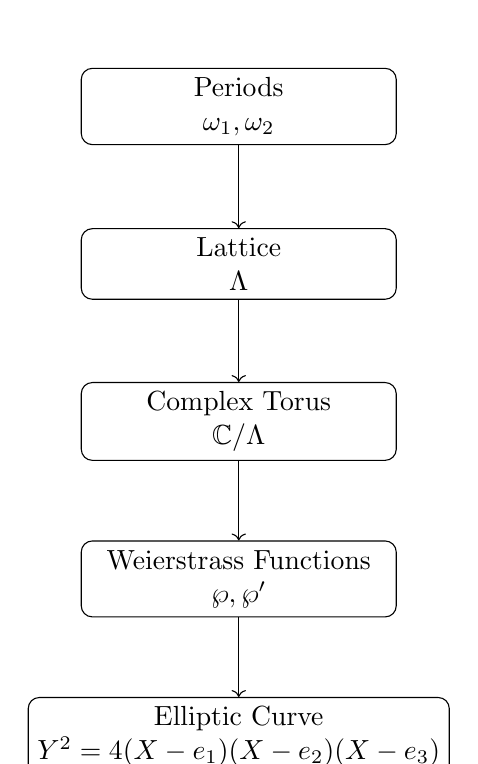
\begin{tikzpicture}[
		node distance=2cm,
		every node/.style={
			draw,
			rounded corners,
			align=center,
			minimum width=4cm
		}
		]
		
		\node (a) {Periods\\ \(\omega_1,\omega_2\)};
		
		\node (b) [below of=a] {Lattice\\ \(\Lambda\)};
		
		\node (c) [below of=b] {Complex Torus\\ \(\mathbb C/\Lambda\)};
		
		\node (d) [below of=c] {Weierstrass Functions\\ \(\wp,\wp'\)};
		
		\node (e) [below of=d] {Elliptic Curve\\ \(Y^2=4(X-e_1)(X-e_2)(X-e_3)\)};
		
		\draw[->] (a)--(b);
		\draw[->] (b)--(c);
		\draw[->] (c)--(d);
		\draw[->] (d)--(e);
		
	\end{tikzpicture}
\end{center}

\section{The Map \texorpdfstring{\(\wp\)}{wp}}

\[
\wp:E=\mathbb C/\Lambda
\longrightarrow
\mathbb P^1
\]

\begin{center}
	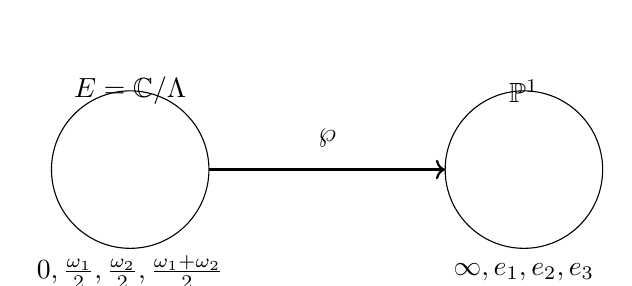
\begin{tikzpicture}[scale=1]
		
		\node at (0,3) {$E=\mathbb C/\Lambda$};
		
		\draw (0,2) circle (1);
		
		\node at (5,3) {$\mathbb P^1$};
		
		\draw (5,2) circle (1);
		
		\draw[->,thick] (1,2)--(4,2);
		
		\node at (2.5,2.4) {$\wp$};
		
		\node at (0,0.7)
		{$0,\frac{\omega_1}{2},\frac{\omega_2}{2},
			\frac{\omega_1+\omega_2}{2}$};
		
		\node at (5,0.7)
		{$\infty,e_1,e_2,e_3$};
		
	\end{tikzpicture}
\end{center}
\section{Concept Map}

\begin{center}
	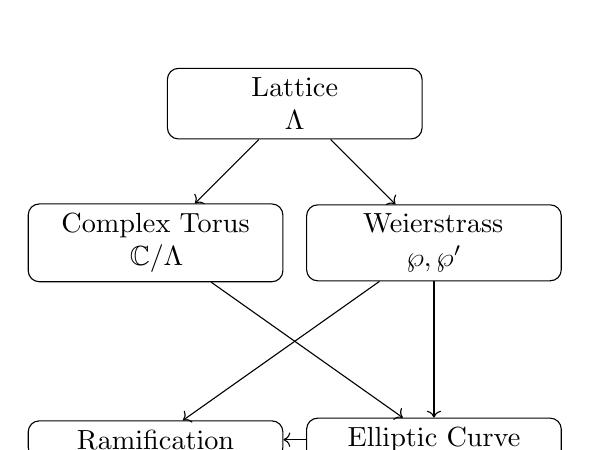
\begin{tikzpicture}[
		node distance=2.5cm,
		every node/.style={
			draw,
			rounded corners,
			align=center,
			text width=3cm
		}
		]
		
		\node (lattice) {Lattice\\ \(\Lambda\)};
		
		\node (torus) [below left of=lattice]
		{Complex Torus\\ \(\mathbb C/\Lambda\)};
		
		\node (wp) [below right of=lattice]
		{Weierstrass\\ \(\wp,\wp'\)};
		
		\node (curve) [below of=wp]
		{Elliptic Curve};
		
		\node (rh) [below of=torus]
		{Ramification};
		
		\draw[->] (lattice)--(torus);
		\draw[->] (lattice)--(wp);
		\draw[->] (torus)--(curve);
		\draw[->] (wp)--(curve);
		\draw[->] (wp)--(rh);
		\draw[->] (curve)--(rh);
		
	\end{tikzpicture}
\end{center}
\section{Related Definitions}

\begin{description}
	
	\item[Lattice]
	A discrete subgroup
	
	\[
	\Lambda=\mathbb Z\omega_1+\mathbb Z\omega_2
	\]
	
	of \(\mathbb C\).
	
	\item[Complex Torus]
	
	The quotient
	
	\[
	\mathbb C/\Lambda.
	\]
	
	A compact Riemann surface of genus one.
	
	\item[Elliptic Function]
	
	A meromorphic function satisfying
	
	\[
	f(z+\lambda)=f(z)
	\]
	
	for all \(\lambda\in\Lambda\).
	
	\item[Weierstrass Function]
	
	The fundamental elliptic function
	
	\[
	\wp(z).
	\]
	
	\item[Half-Period]
	
	One of
	
	\[
	\frac{\omega_1}{2},
	\quad
	\frac{\omega_2}{2},
	\quad
	\frac{\omega_1+\omega_2}{2}.
	\]
	
	\item[Branch Point]
	
	A value where several sheets of a covering come together.
	
	\item[Ramification Point]
	
	A point where a holomorphic map is not locally injective.
	
	\item[Elliptic Curve]
	
	A smooth cubic curve
	
	\[
	Y^2=4X^3-g_2X-g_3.
	\]
	
	\item[Riemann--Hurwitz Formula]
	
	\[
	2g_X-2
	=
	d(2g_Y-2)
	+
	\sum(e_p-1).
	\]
	
	Relates genus, degree and ramification.
	
\end{description}

\end{document}

